
\DIFaddbegin 

\clearpage
\subsection{\DIFadd{The  Bone and Antler merchant}}
\label{sec:appendix:moj:bone}

\DIFadd{Bone was used a lot for carving objects like buckles. Antler was used for objects like combs that needed to be stronger. If available, these tradesmen would also use horn and ivory.
}

\begin{display}{The  bone and antler stall}
	\label{fig:appendix:moj:places:bone:stall}
	\DIFadd{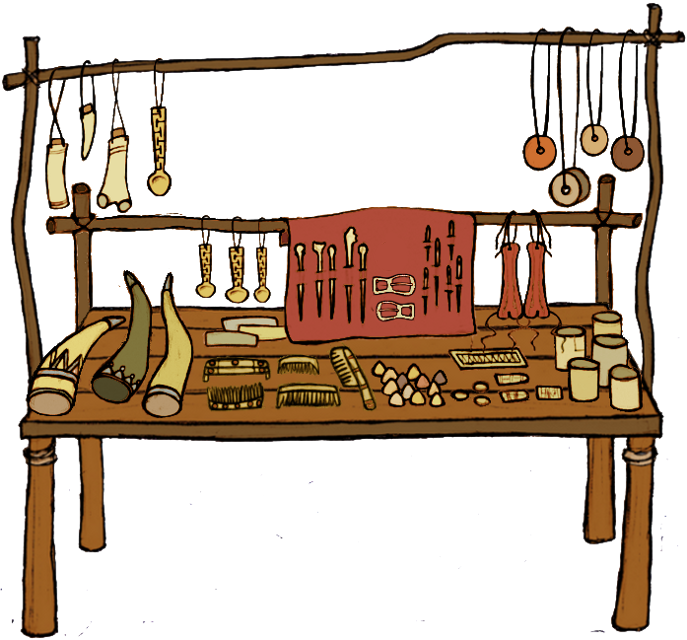
\includegraphics[width=0.65\columnwidth]{img/Jorvik/places/bone stall}
}\end{display}

\begin{display}{The  bone and antler stall with a background and a merchant}
	\label{fig:appendix:moj:places:bone}
	\DIFadd{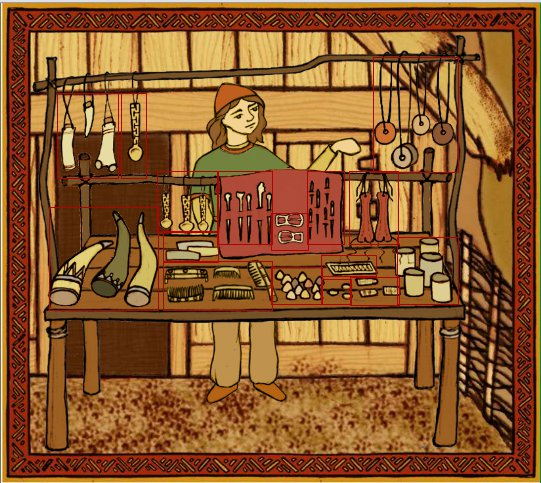
\includegraphics[width=0.65\columnwidth]{img/Jorvik/places/bone}
}\end{display}
\clearpage


\begin{table}[ht!]
	\centering
	\begin{tabular}{ p{3cm} c }\toprule
		\textbf{\DIFaddFL{Name:}} & \multirow{5}{*}{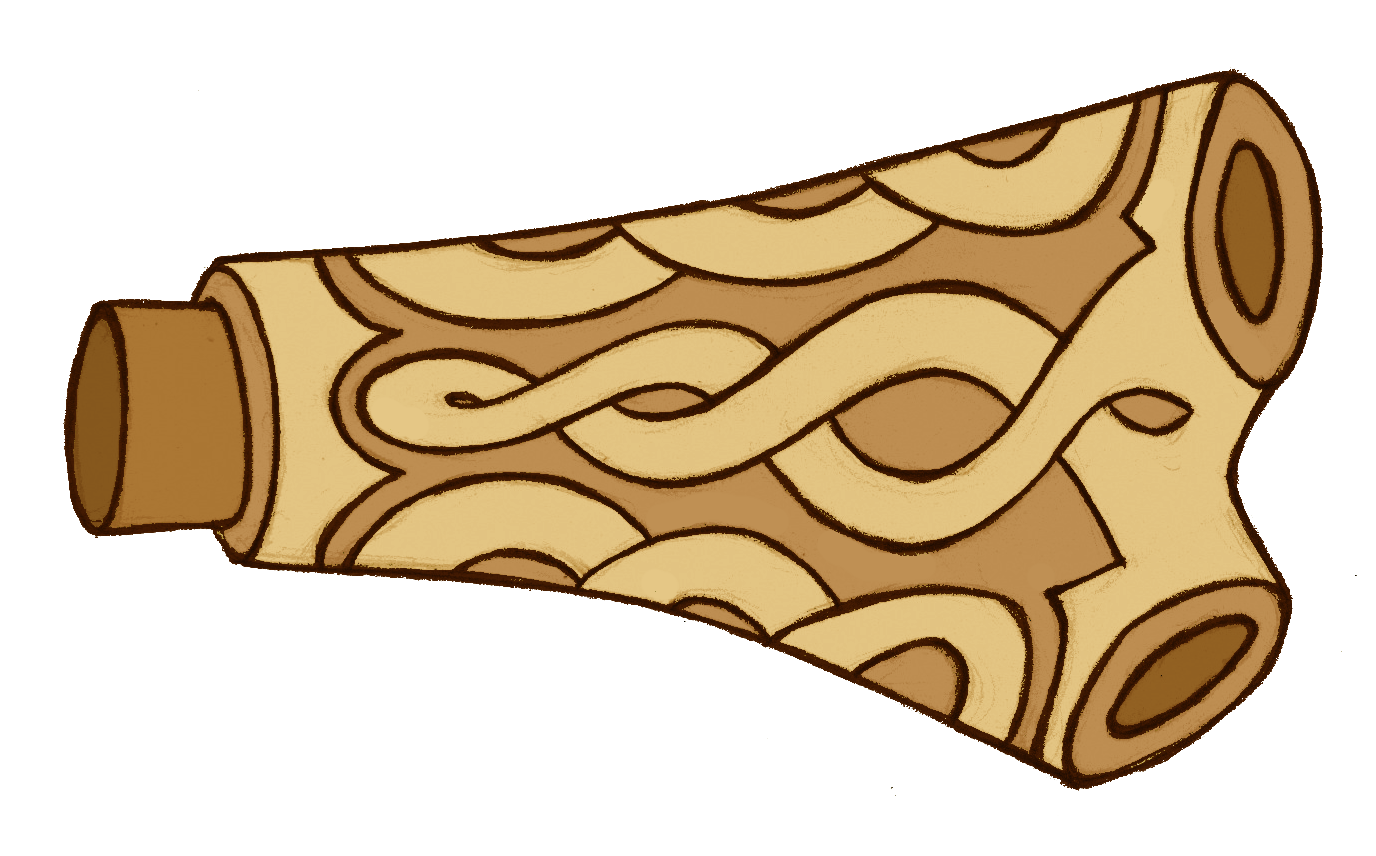
\includegraphics[height=30mm]{img/Jorvik/objects/bone/vial}}\\
		\DIFaddFL{Vial }& \\ 
		\textbf{\DIFaddFL{Price:}} & \\
		\DIFaddFL{1.32 silver }& \\ 
		\textbf{\DIFaddFL{Description:}} & \\
		\multicolumn{2}{p{12cm}}{Vials were made out of bone and were used to store herbs, pepper and spices. Spices were very expensive so they would need to be kept safe and dry to keep their taste and quality.}\\
		\bottomrule
	\end{tabular}
\end{table}

\begin{table}[ht!]
	\centering
	\begin{tabular}{ p{3cm} c }\toprule
		\textbf{\DIFaddFL{Name:}} & \multirow{5}{*}{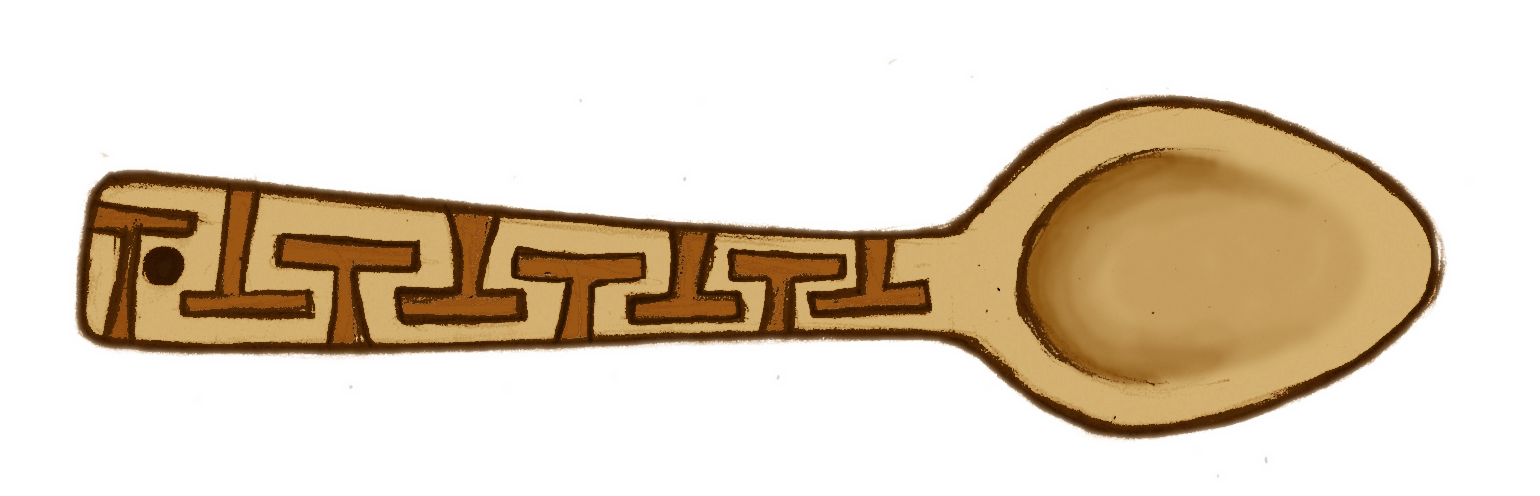
\includegraphics[width=70mm]{img/Jorvik/objects/bone/spoon}}\\
		\DIFaddFL{Spoon }& \\ 
		\textbf{\DIFaddFL{Price:}} & \\
		\DIFaddFL{0.88 silver }& \\ 
		\textbf{\DIFaddFL{Description:}} & \\
		\multicolumn{2}{p{12cm}}{Vikings didn't have forks so they ate using spoons, made from bone or wood. If food needed cutting, they used a sharp metal knife.}\\
		\bottomrule
	\end{tabular}
\end{table}

\begin{table}[ht!]
	\centering
	\begin{tabular}{ p{3cm} c }\toprule
		\textbf{\DIFaddFL{Name:}} & \multirow{5}{*}{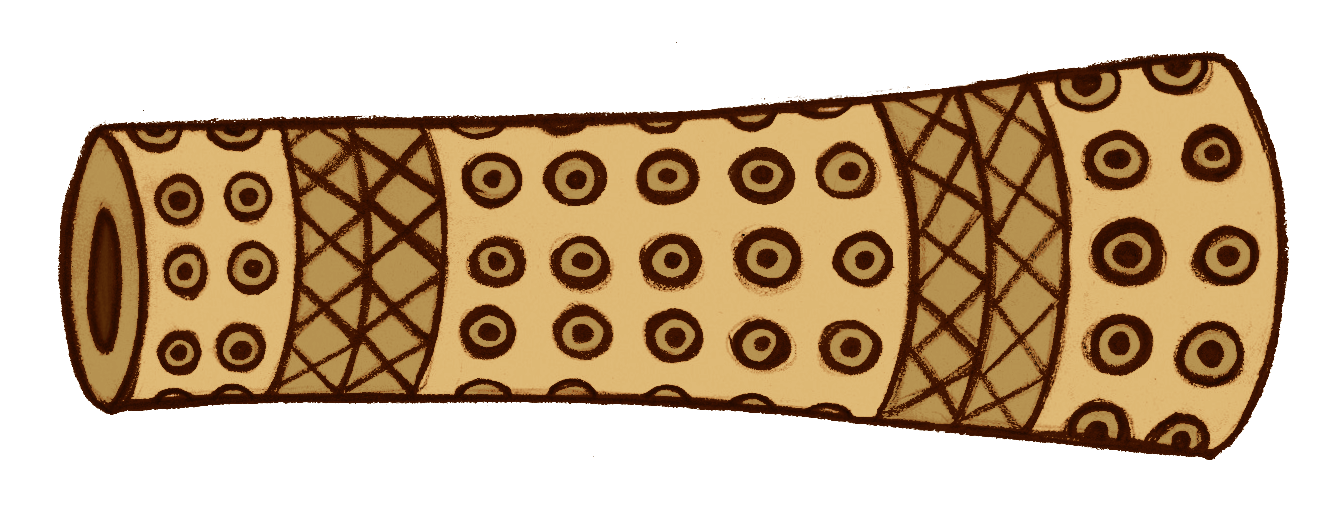
\includegraphics[width=70mm]{img/Jorvik/objects/bone/handle}}\\
		\DIFaddFL{Handle }& \\ 
		\textbf{\DIFaddFL{Price:}} & \\
		\DIFaddFL{2.64 silver }& \\ 
		\textbf{\DIFaddFL{Description:}} & \\
		\multicolumn{2}{p{12cm}}{Vikings often used antler or wood to make handles for objects like knives. They would be decorated to add value.}\\
		\bottomrule
	\end{tabular}
\end{table}

\begin{table}[ht!]
	\centering
	\begin{tabular}{ p{3cm} c }\toprule
		\textbf{\DIFaddFL{Name:}} & \multirow{5}{*}{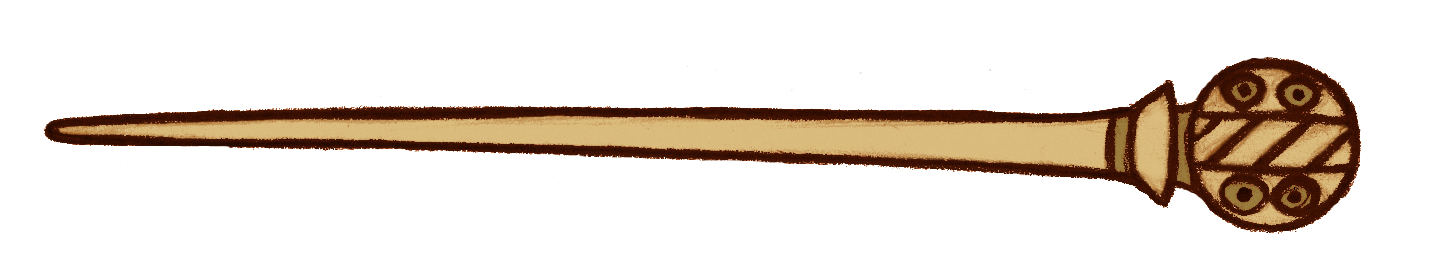
\includegraphics[width=70mm]{img/Jorvik/objects/bone/pin}}\\
		\DIFaddFL{Pin }& \\ 
		\textbf{\DIFaddFL{Price:}} & \\
		\DIFaddFL{1.32 silver }& \\ 
		\textbf{\DIFaddFL{Description:}} & \\
		\multicolumn{2}{p{12cm}}{Vikings used pins to fasten their clothing. The Jorvik dig at Coppergate has unearthed many pins that are made from the tibia (shinbone) of pigs.}\\
		\bottomrule
	\end{tabular}
\end{table}

\begin{table}[ht!]
	\centering
	\begin{tabular}{ p{3cm} c }\toprule
		\textbf{\DIFaddFL{Name:}} & \multirow{5}{*}{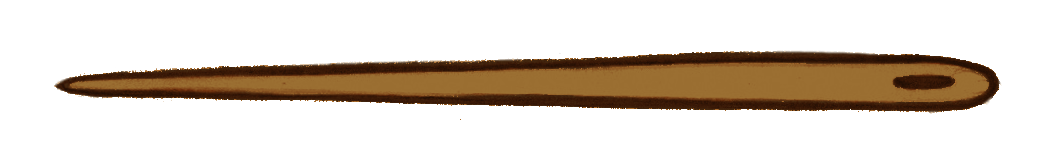
\includegraphics[width=70mm]{img/Jorvik/objects/bone/needle}}\\
		\DIFaddFL{Needle }& \\ 
		\textbf{\DIFaddFL{Price:}} & \\
		\DIFaddFL{1.76 silver }& \\ 
		\textbf{\DIFaddFL{Description:}} & \\
		\multicolumn{2}{p{12cm}}{Vikings had several methods for making clothes. Naalbinding was used to knit socks using only one needle. }\\
		\bottomrule
	\end{tabular}
\end{table}

\begin{table}[ht!]
	\centering
	\begin{tabular}{ p{3cm} c }\toprule
		\textbf{\DIFaddFL{Name:}} & \multirow{5}{*}{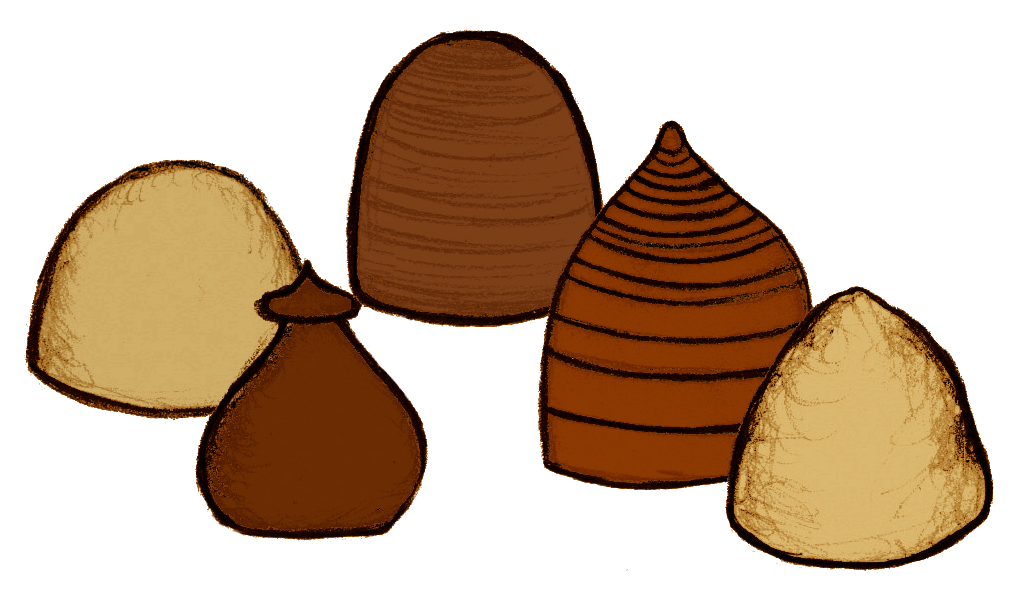
\includegraphics[height=30mm]{img/Jorvik/objects/bone/game pieces}}\\
		\DIFaddFL{Game Pieces }& \\ 
		\textbf{\DIFaddFL{Price:}} & \\
		\DIFaddFL{7.50 silver }& \\ 
		\textbf{\DIFaddFL{Description:}} & \\
		\multicolumn{2}{p{12cm}}{Richer Vikings could have specially crafted game pieces for their strategy board games similar to chess, but coloured pebbles worked just as well.}\\
		\bottomrule
	\end{tabular}
\end{table}

\begin{table}[ht!]
	\centering
	\begin{tabular}{ p{3cm} c }\toprule
		\textbf{\DIFaddFL{Name:}} & \multirow{5}{*}{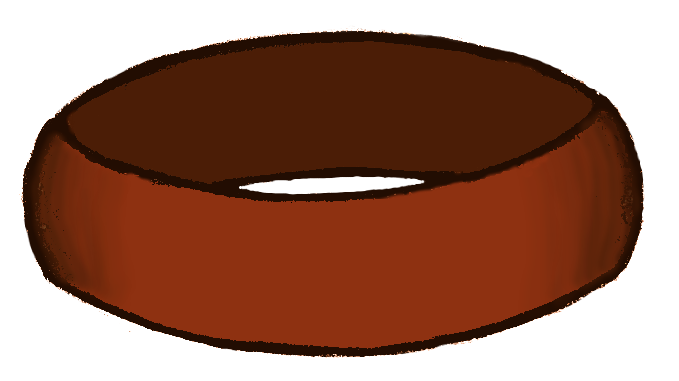
\includegraphics[height=30mm]{img/Jorvik/objects/bone/ring}}\\
		\DIFaddFL{Ring }& \\ 
		\textbf{\DIFaddFL{Price:}} & \\
		\DIFaddFL{2.21 silver }& \\ 
		\textbf{\DIFaddFL{Description:}} & \\
		\multicolumn{2}{p{12cm}}{Rings could be made from a range of materials depending on the wealth of the customer. They could be made of wood, bone, metal, glass or even amber that came from the Baltic region.}\\
		\bottomrule
	\end{tabular}
\end{table}

\begin{table}[ht!]
	\centering
	\begin{tabular}{ p{3cm} c }\toprule
		\textbf{\DIFaddFL{Name:}} & \multirow{5}{*}{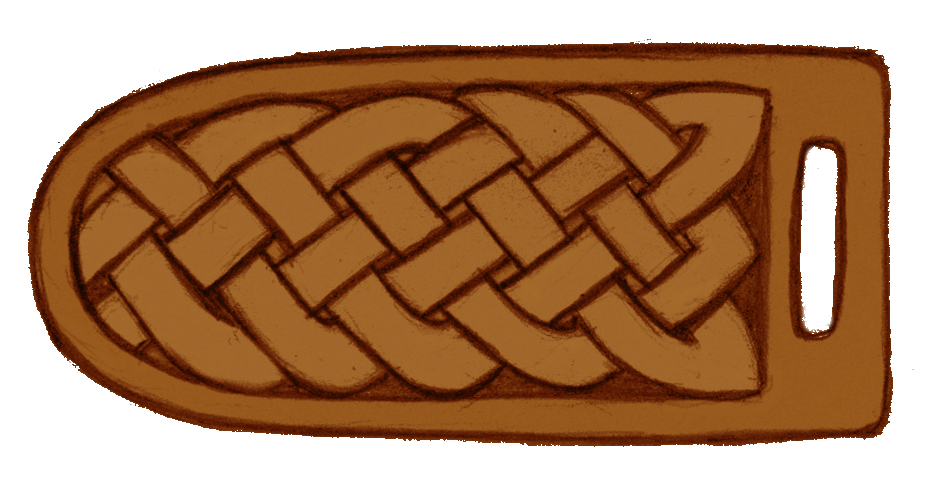
\includegraphics[height=30mm]{img/Jorvik/objects/bone/strap ends}}\\
		\DIFaddFL{Strap Ends }& \\ 
		\textbf{\DIFaddFL{Price:}} & \\
		\DIFaddFL{2.65 silver }& \\ 
		\textbf{\DIFaddFL{Description:}} & \\
		\multicolumn{2}{p{12cm}}{Strap ends could be made from antler, bone or metal but not all belts had them. They were a status symbol to show that you were wealthy.}\\
		\bottomrule
	\end{tabular}
\end{table}

\begin{table}[ht!]
	\centering
	\begin{tabular}{ p{3cm} c }\toprule
		\textbf{\DIFaddFL{Name:}} & \multirow{5}{*}{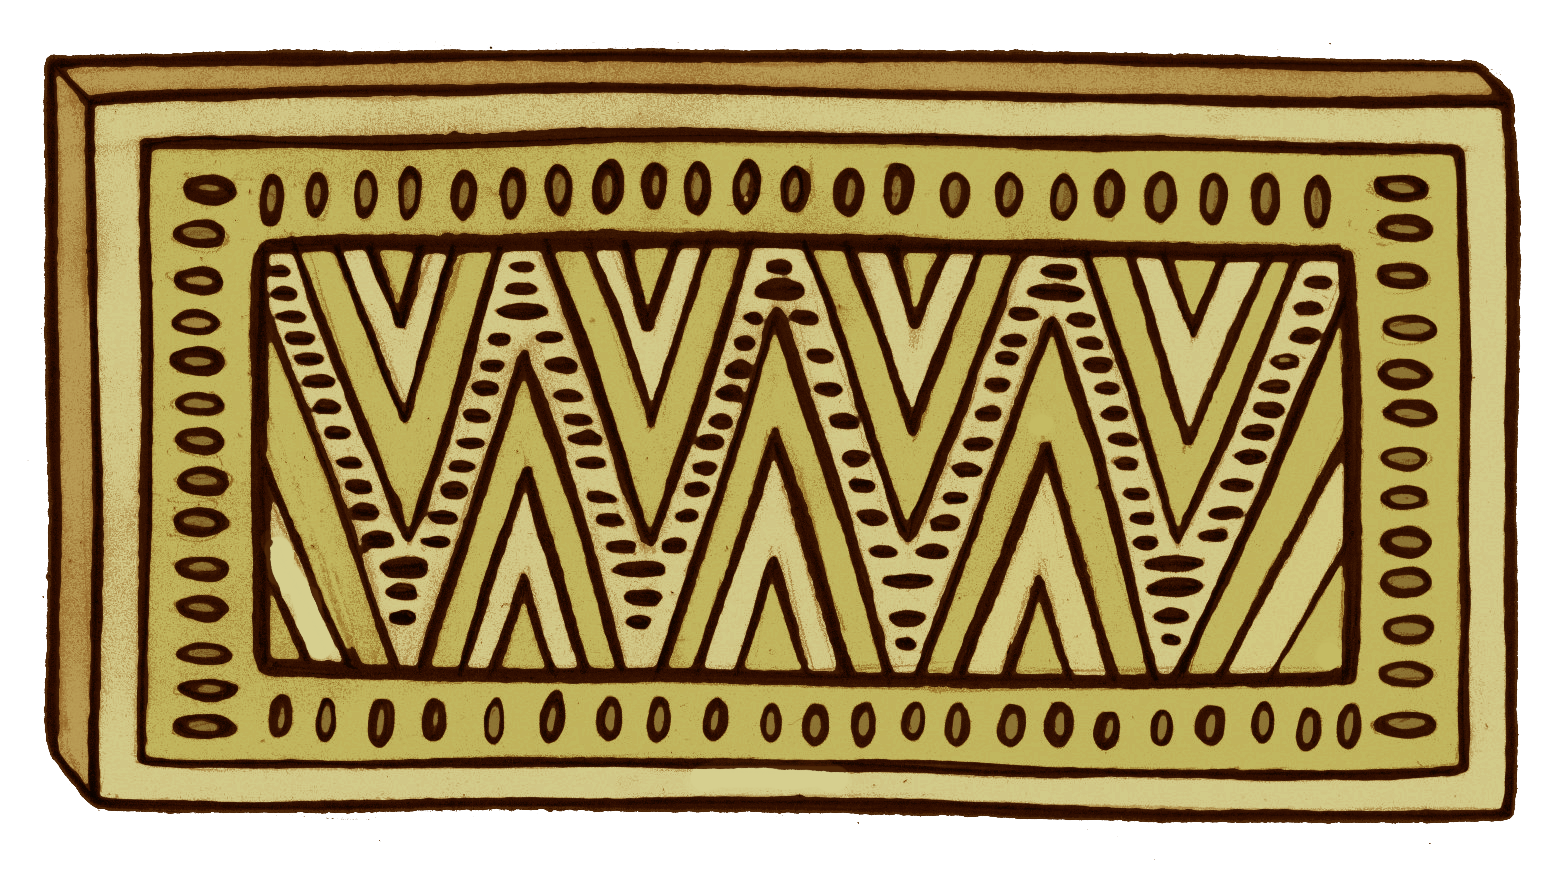
\includegraphics[height=30mm]{img/Jorvik/objects/bone/decorative plate}}\\
		\DIFaddFL{Decorative Plate }& \\ 
		\textbf{\DIFaddFL{Price:}} & \\
		\DIFaddFL{3.97 silver }& \\ 
		\textbf{\DIFaddFL{Description:}} & \\
		\multicolumn{2}{p{12cm}}{A decorative plate was a panel of patterned bone that could be attached to an object like a chest to make it look more attractive. The Vikings took a lot of pride in their appearance and that of their possessions.}\\
		\bottomrule
	\end{tabular}
\end{table}

\begin{table}[ht!]
	\centering
	\begin{tabular}{ p{3cm} c }\toprule
		\textbf{\DIFaddFL{Name:}} & \multirow{5}{*}{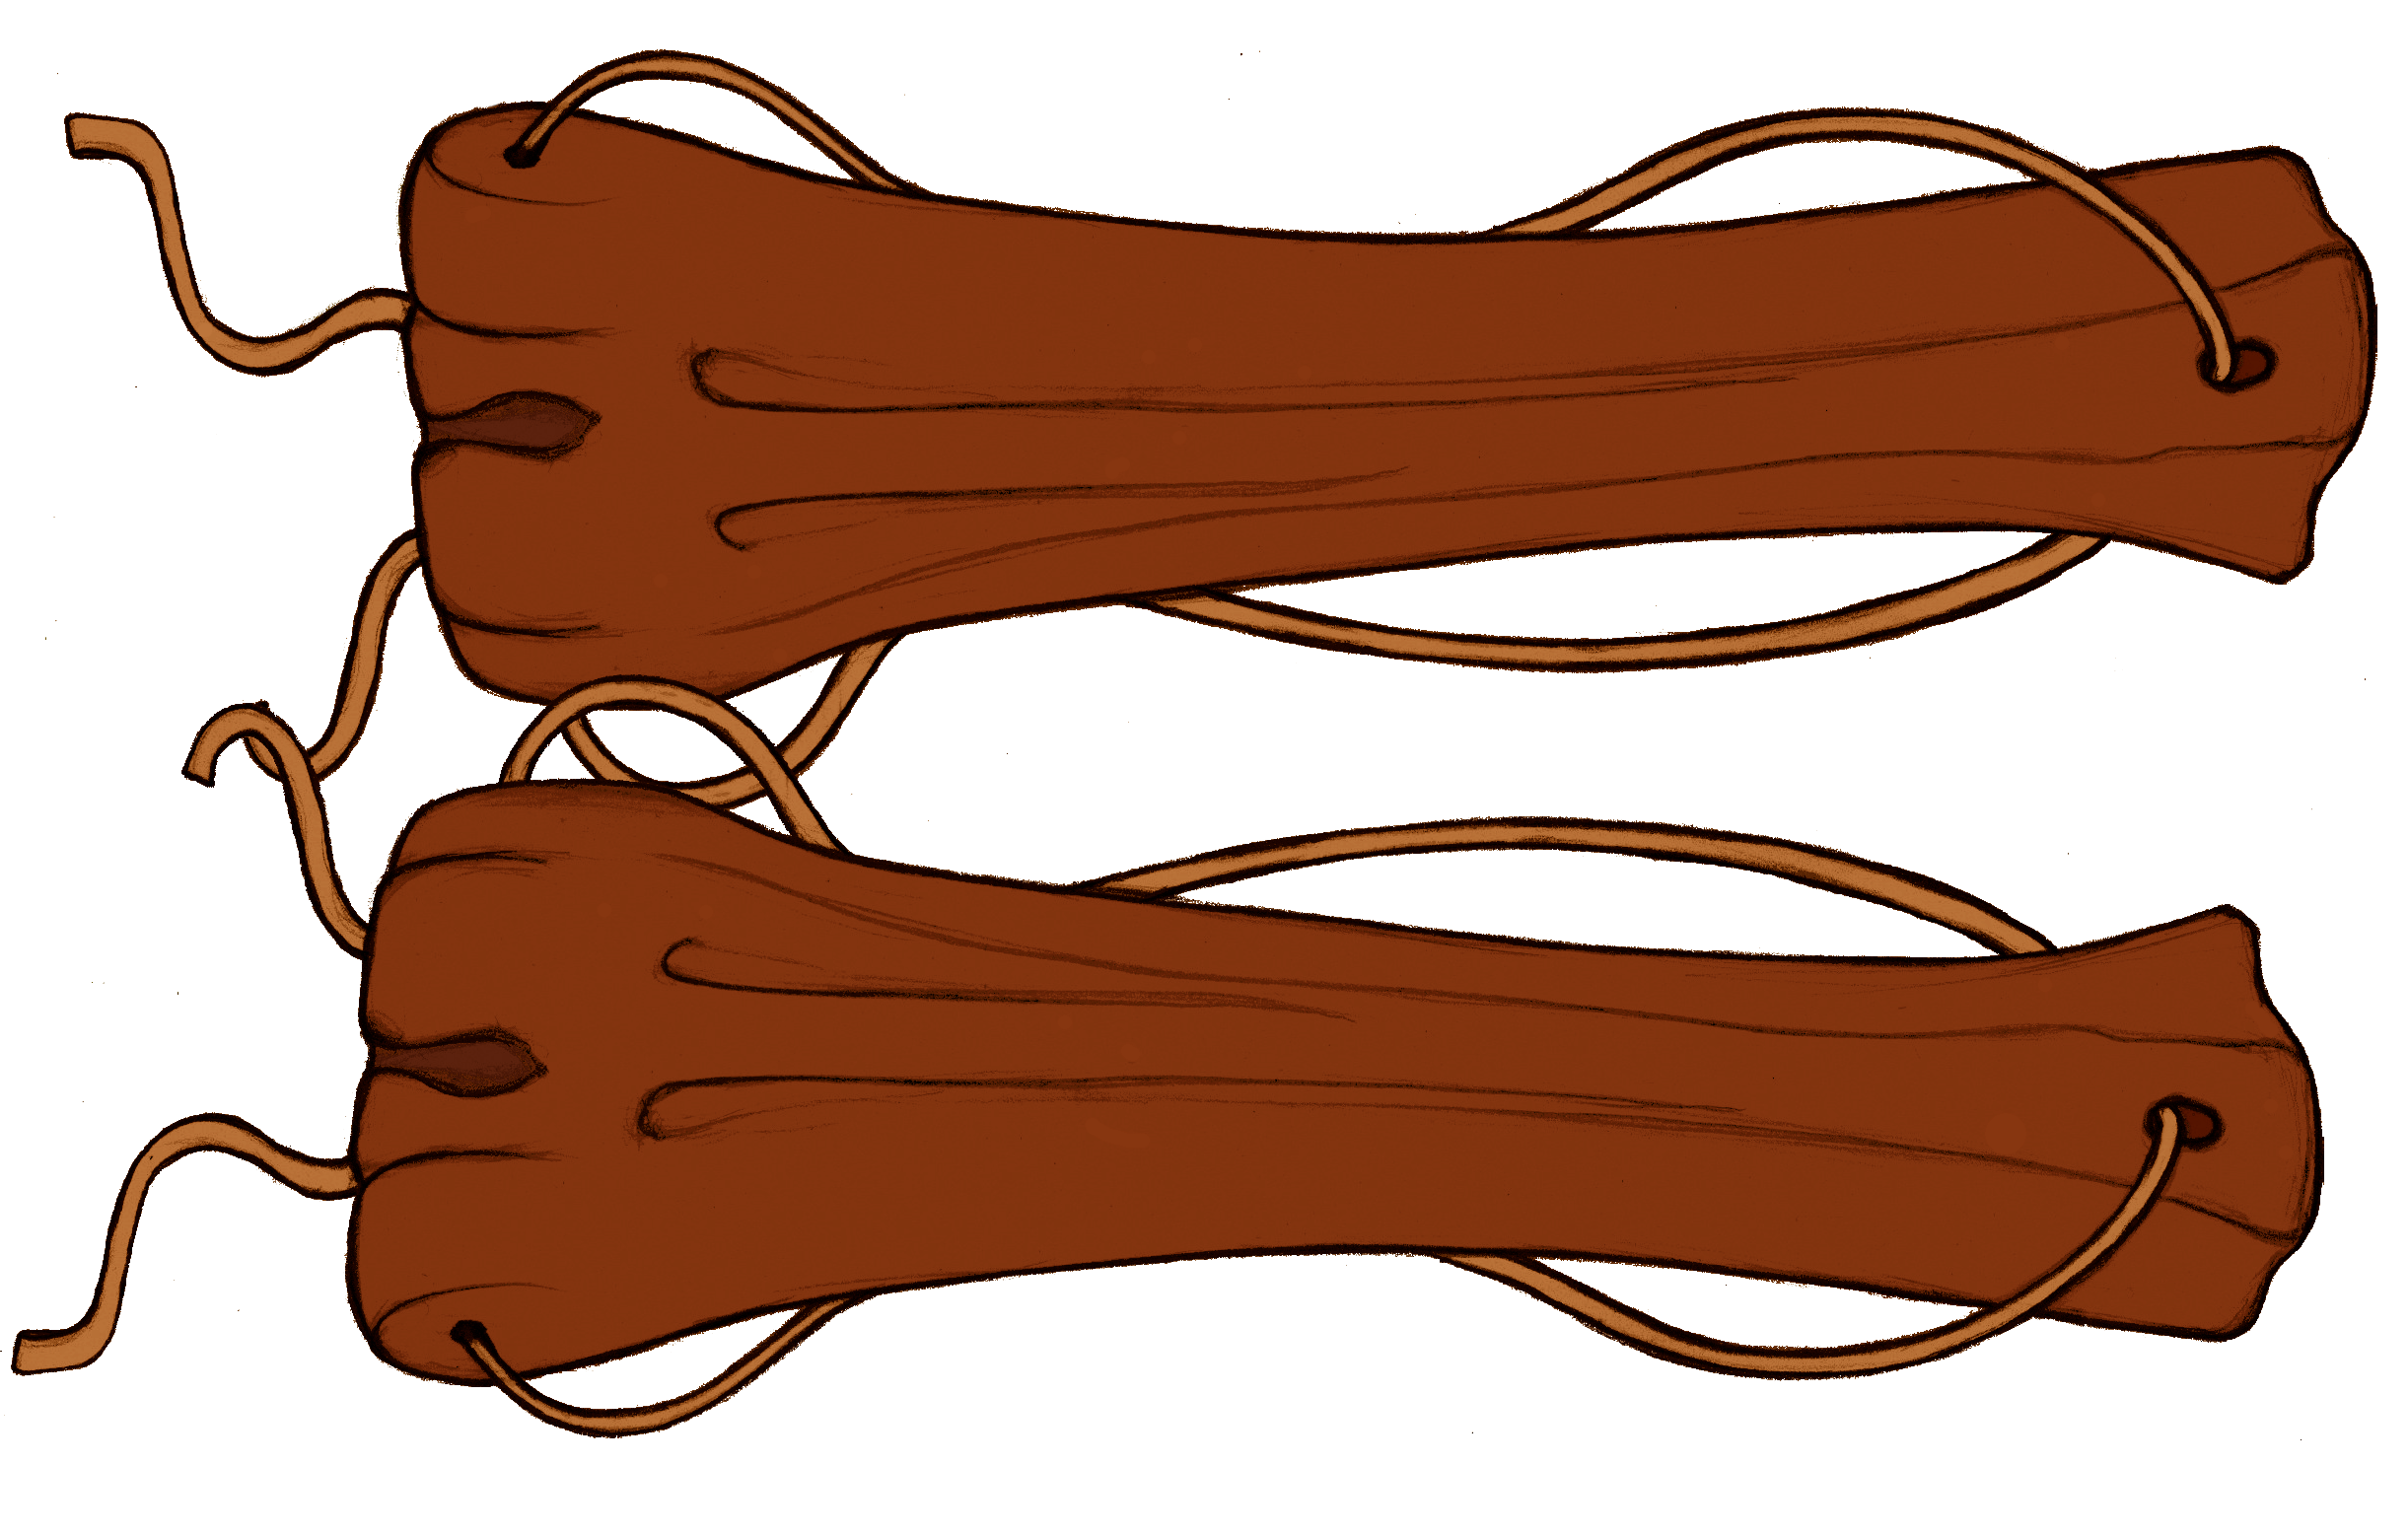
\includegraphics[height=30mm]{img/Jorvik/objects/bone/ice skates}}\\
		\DIFaddFL{Ice Skates }& \\ 
		\textbf{\DIFaddFL{Price:}} & \\
		\DIFaddFL{6.62 silver }& \\ 
		\textbf{\DIFaddFL{Description:}} & \\
		\multicolumn{2}{p{12cm}}{Skates were made from a horse's shinbone. They would have been tied to shoes using a leather thong to make it easier to cross icy and slippery surfaces.}\\
		\bottomrule
	\end{tabular}
\end{table}

\begin{table}[ht!]
	\centering
	\begin{tabular}{ p{3cm} c }\toprule
		\textbf{\DIFaddFL{Name:}} & \multirow{5}{*}{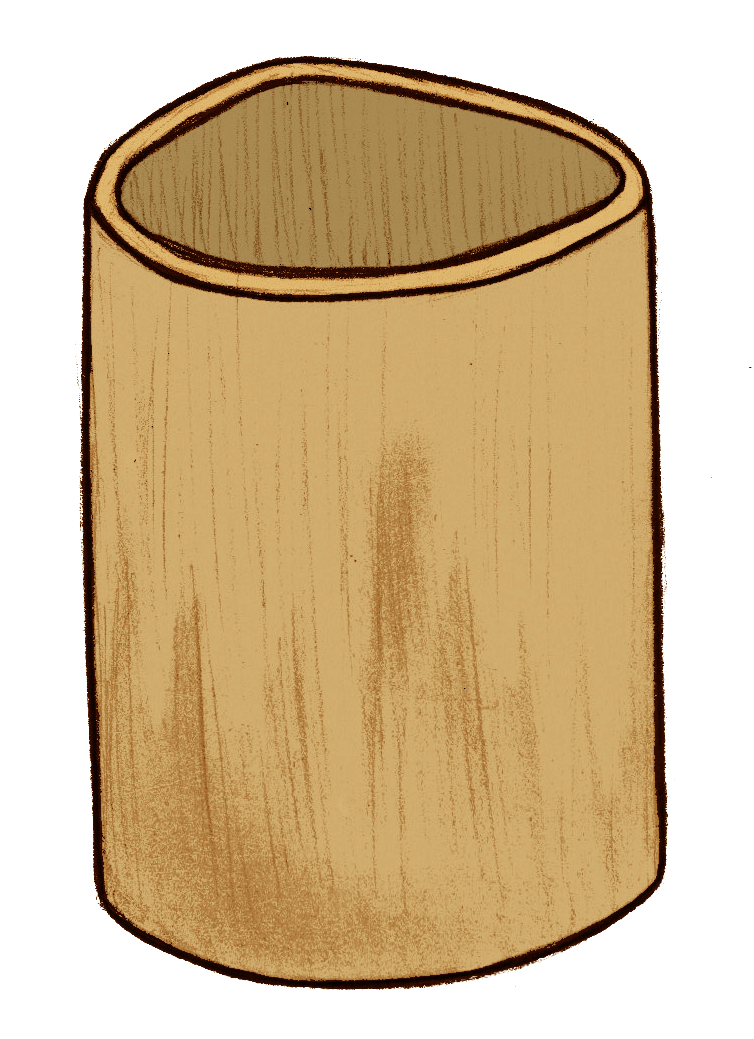
\includegraphics[height=30mm]{img/Jorvik/objects/bone/cup}}\\
		\DIFaddFL{Cup }& \\ 
		\textbf{\DIFaddFL{Price:}} & \\
		\DIFaddFL{1.32 silver }& \\ 
		\textbf{\DIFaddFL{Description:}} & \\
		\multicolumn{2}{p{12cm}}{Cups could be made from a range of materials including wood, clay or cow horn. They rarely had handles so would resemble beakers rather than mugs.}\\
		\bottomrule
	\end{tabular}
\end{table}

\begin{table}[ht!]
	\centering
	\begin{tabular}{ p{3cm} c }\toprule
		\textbf{\DIFaddFL{Name:}} & \multirow{5}{*}{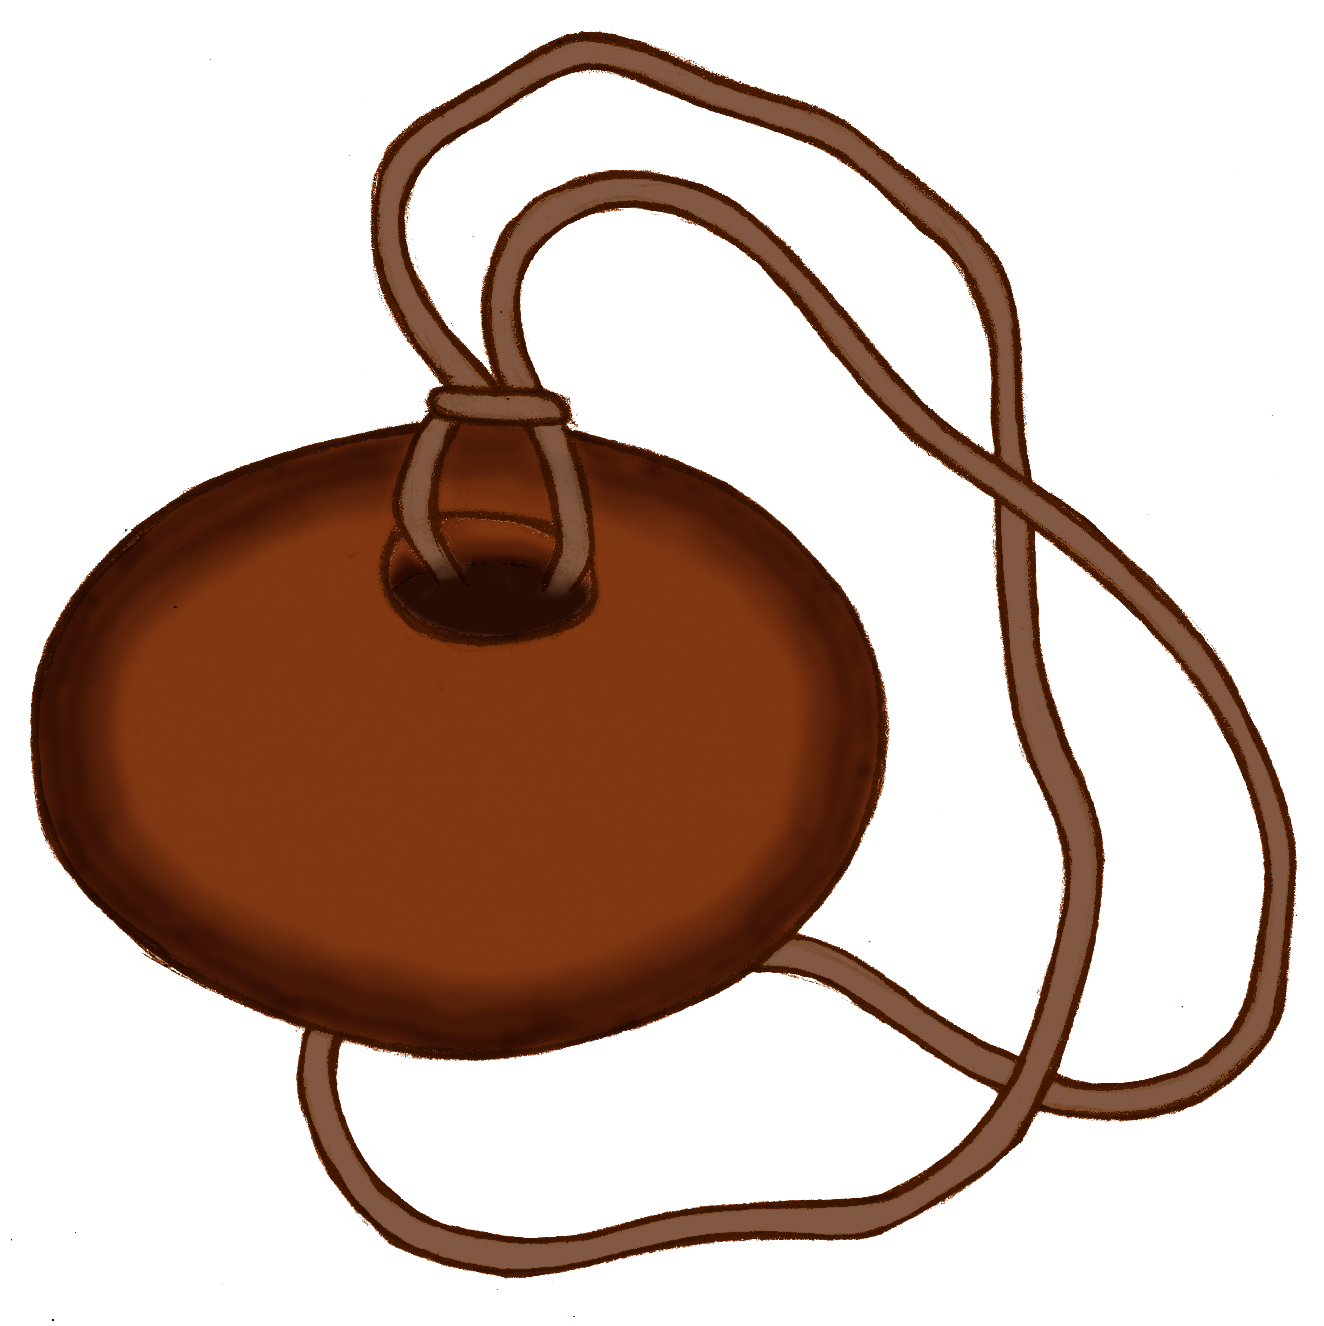
\includegraphics[height=30mm]{img/Jorvik/objects/bone/spindle whorl}}\\
		\DIFaddFL{Spindle Whorl }& \\ 
		\textbf{\DIFaddFL{Price:}} & \\
		\DIFaddFL{3.08 silver }& \\ 
		\textbf{\DIFaddFL{Description:}} & \\
		\multicolumn{2}{p{12cm}}{Spindle whorls could be made from antler or bone, but also amber, clay, wood, metal or any type of stone that could be found! They were frequently buried with women after death.}\\
		\bottomrule
	\end{tabular}
\end{table}

\begin{table}[ht!]
	\centering
	\begin{tabular}{ p{3cm} c }\toprule
		\textbf{\DIFaddFL{Name:}} & \multirow{5}{*}{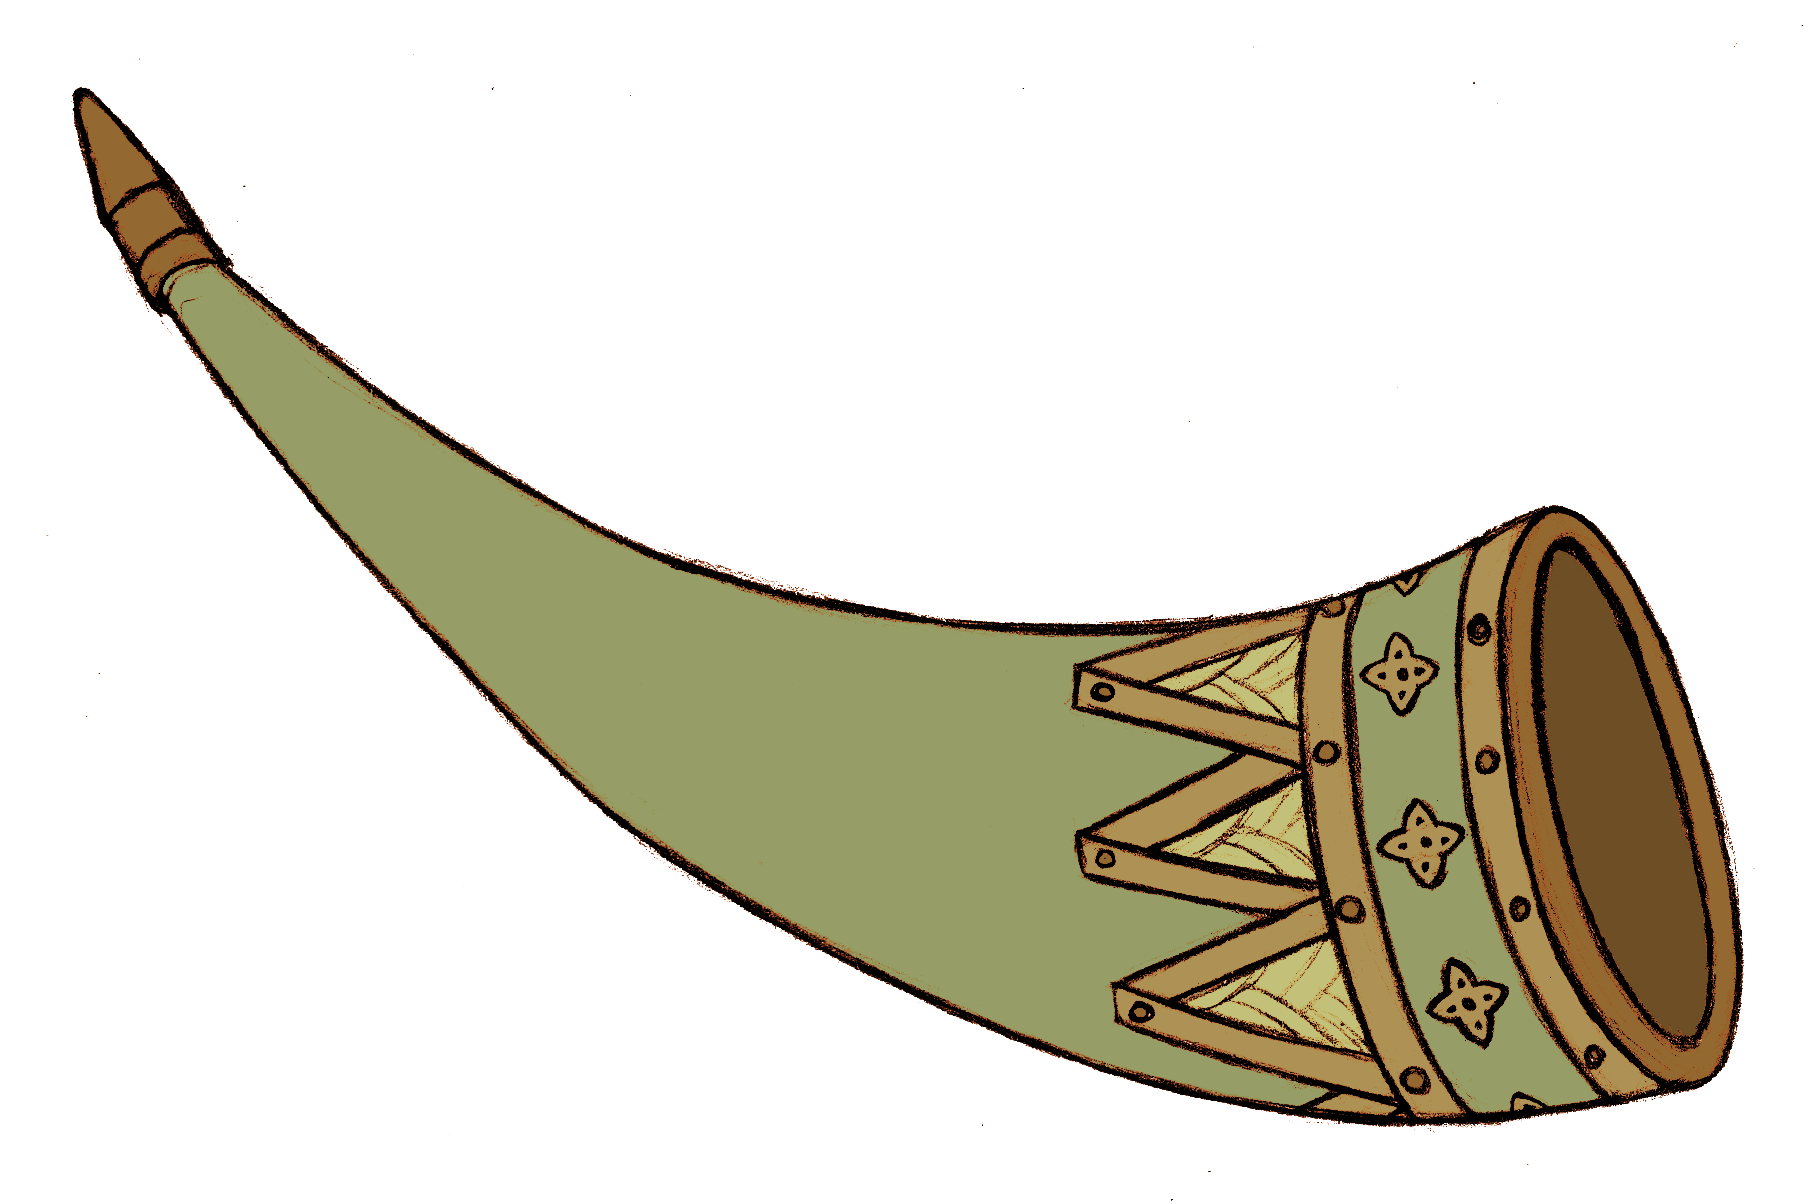
\includegraphics[height=30mm]{img/Jorvik/objects/bone/drinking horn}}\\
		\DIFaddFL{Drinking Horn }& \\ 
		\textbf{\DIFaddFL{Price:}} & \\
		\DIFaddFL{1.76 silver }& \\ 
		\textbf{\DIFaddFL{Description:}} & \\
		\multicolumn{2}{p{12cm}}{Vikings drank from the horns. Because there was no easy way to put it down, the horn would be passed from person to person until it was empty.}\\
		\bottomrule
	\end{tabular}
\end{table}

\begin{table}[ht!]
	\centering
	\begin{tabular}{ p{3cm} c }\toprule
		\textbf{\DIFaddFL{Name:}} & \multirow{5}{*}{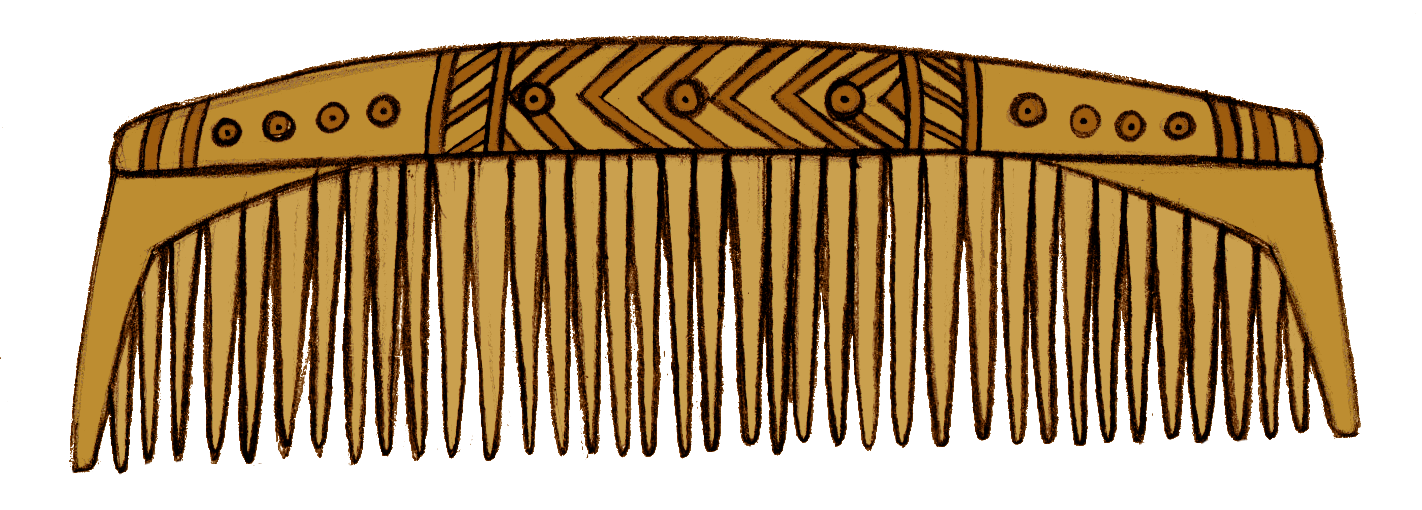
\includegraphics[width=70mm]{img/Jorvik/objects/bone/comb}}\\
		\DIFaddFL{Comb }& \\ 
		\textbf{\DIFaddFL{Price:}} & \\
		\DIFaddFL{3.52 silver }& \\ 
		\textbf{\DIFaddFL{Description:}} & \\
		\multicolumn{2}{p{12cm}}{Combs would have been made from antler or occasionally bone. Vikings took a lot of pride in their appearance taking care to wash and comb their hair.}\\
		\bottomrule
	\end{tabular}
\end{table}

\begin{table}[ht!]
	\centering
	\begin{tabular}{ p{3cm} c }\toprule
		\textbf{\DIFaddFL{Name:}} & \multirow{5}{*}{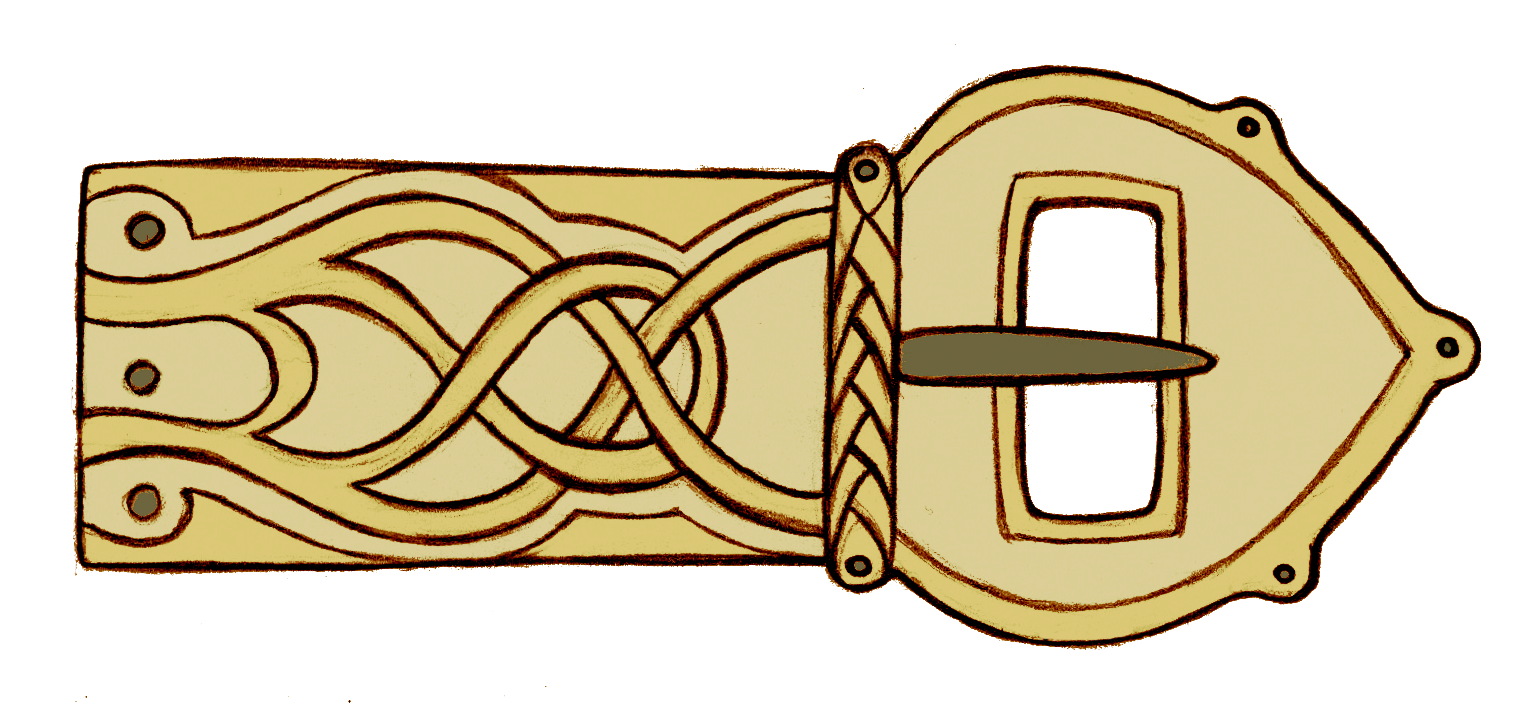
\includegraphics[height=30mm]{img/Jorvik/objects/bone/buckle}}\\
		\DIFaddFL{Buckle }& \\ 
		\textbf{\DIFaddFL{Price:}} & \\
		\DIFaddFL{2.20 silver }& \\ 
		\textbf{\DIFaddFL{Description:}} & \\
		\multicolumn{2}{p{12cm}}{Buckles could be made of metal or bone. Like many Viking objects, it would have been carved with patterns to make it more decorative.}\\
		\bottomrule
	\end{tabular}
\end{table} \DIFaddend